\chapter{Map navigation}

\pagestyle{fancy}
\fancyhf{}
\fancyhead[OC]{\leftmark}
\fancyhead[EC]{\rightmark}
%\renewcommand{\footrulewidth}{1pt}
\cfoot{\thepage}


Play about with the map canvas view:
\begin{enumerate}[~~~1)]
	\item
	See the Co-ordinates change in status bar as move mouse
	\item
	Use the icons in the \textit{Map Navigation Toolbar}: Pan, Zoom (in, out, full, layer, backward, forward). Can also use the mouse wheel to zoom (use ctrl key for finer control).\\
	Any yellow on an icon indicates that it is about selected features (we will visit this later).\\ %	let's use the \textit{Attributes Toolbar} to select features).
	\textit{Zoom to Layer} is a frequently used feature, which can also be accessed by right clicking the layer in the Layers Panel, and selecting the top option \textit{Zoom to Layer}.
	\begin{figure}[!h]
		\centering
		
\includegraphics[width=0.5\textwidth]{images/map_navigation_toolbar_icons.png}
		\caption{Map Navigation Toolbar icons}
		\label{ft_fig_firstfig3}
	\end{figure}
	\item 
	The scale in the \textit{Status Bar} (at the bottom of the window) changes as you zoom 
	\begin{tabular}{@{}c@{}}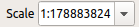
\includegraphics[width=8ex]{images/scale_status_bar.png}\end{tabular}
	. Can type the desired scale.
	\item
	\textit{Bookmarking} 
	\begin{tabular}{@{}c@{}}
\includegraphics[width=4ex]{images/bookmark_icons.png}\end{tabular}
	specific map views so can revisit them easily (this opens the relevant \textit{Spatial Bookmarks Panel})
	\begin{figure}[!h]
		\centering
		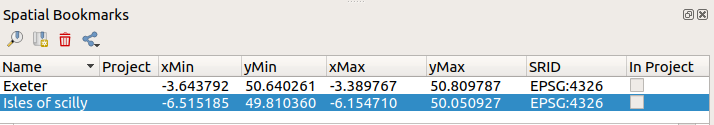
\includegraphics[width=0.5\textwidth]{images/spatial_bookmarks_panel.png}
		\caption{Spatial bookmarks panel with two saved map views}
		\label{ft_fig_firstfig3}
	\end{figure}
	\item
	\textit{Map Views} are useful when comparing two or more areas. Select the New Map View icon 
	\begin{tabular}{@{}c@{}}
\includegraphics[width=4ex]{images/new_map_view_icon.png}\end{tabular}
	to create a pop-up window that are independent of the main window view. Can dock these sub-windows to the side of the main window.
	
	\begin{figure}[!h]
		\centering
		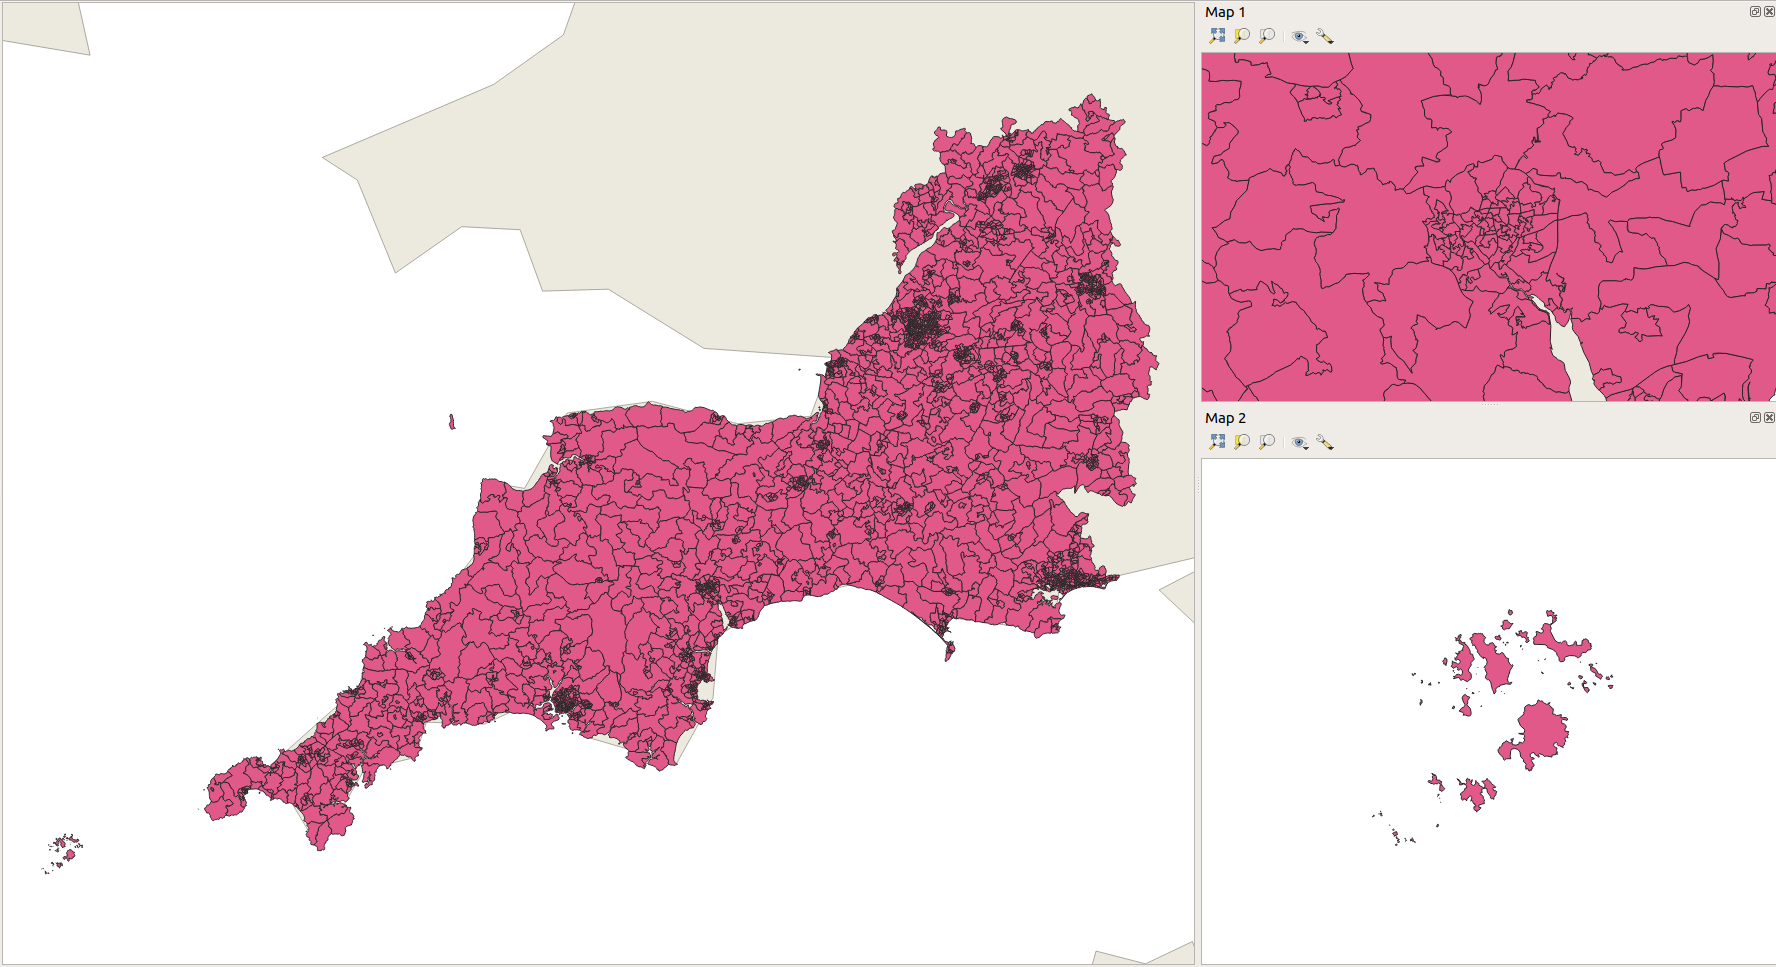
\includegraphics[width=0.4\textwidth]{images/three_map_views.png}
		\caption{Map canvas on left with two map views docked to the right of the window}
		\label{ft_fig_firstfig3}
	\end{figure}
	
\end{enumerate}